\documentclass[10pt,a4paper]{article}
\usepackage[utf8]{inputenc}
\usepackage[T1]{fontenc}
\usepackage{amsmath}
\usepackage{amsfonts}
\usepackage{amssymb}

\usepackage{listings}
\usepackage{color}
\usepackage{tikz}
\usetikzlibrary{arrows}
\usepackage{hyperref}

\title{DD2200 - Operativsystem \\ Laboration 1 \\ Digenv - processkommunikation med pipes  v1.1 \\ Period 1, läsår 2014}
\author{Carl Svensson, F-10 \\ 910414-1412 \\ carlsven@kth.se}
\date{}

\definecolor{dkgreen}{rgb}{0,0.6,0}
\definecolor{gray}{rgb}{0.5,0.5,0.5}
\definecolor{mauve}{rgb}{0.58,0,0.82}

\lstdefinestyle{cstyle}{%
  language=C,
  aboveskip=3mm,
  belowskip=3mm,
  showstringspaces=false,
  columns=flexible,
  basicstyle={\small\ttfamily},
  numbers=none,
  numberstyle=\color{mauve},
  keywordstyle=\color{blue},
  commentstyle=\color{dkgreen},
  stringstyle=\color{mauve},
  breaklines=true,
  breakatwhitespace=true
  tabsize=3
}

\lstdefinestyle{bashstyle}{%
  language=C,
  aboveskip=3mm,
  belowskip=3mm,
  showstringspaces=false,
  columns=flexible,
  basicstyle={\small\ttfamily},
  numbers=none,
  numberstyle=\color{mauve},
  keywordstyle=\color{blue},
  commentstyle=\color{dkgreen},
  stringstyle=\color{mauve},
  breaklines=true,
  breakatwhitespace=true
  tabsize=3
}

\lstset{
  style=bashstyle
}

\begin{document}

\maketitle
\tableofcontents
\clearpage


\section{Problembeskrivning}

Uppgiften är att skriva ett program som underlättar att titta på miljövariablerna. Programmet ska motsvara att köra "printenv | grep <filter> | sort | less" i t.ex. Bash. Om inget filter anges så hoppas grep-steget över.
Programmet ska dessutom inte nödvändigtvis använda just \emph{less} utan det program som är satt som pager. Detta hittas med hjälp av PAGER-miljövariabeln. Om den inte är satt så används \emph{less} men om den inte finns så ska istället \emph{more} användas.

\subsection{Förberedelsefrågor}

\begin{enumerate}
\item Processen med pid $1$ heter \emph{init}
\item Barnprocesser ärver en kopia av föräldraprocessens alla miljövariabler vilket gör att man kan kommunicera från föräldraprocess till barnprocess med dem. Det går däremot inte att kommunicera åt andra hållet med dem.
\item Anrop till \emph{sigaction} med \emph{SIGKILL} som argument resulterar i ett felmeddelande "Invalid argument". Man-sidan specificerar tydligt att man inte kan anropa \emph{sigaction} med bland annat \emph{SIGKILL} som argument och att det i så fall genererar felkoden \emph{EINVAL}. 
\item Föräldraprocessen måste kunna veta PID till barnprocessen och får därför den från fork. Om barnprocessen behöver veta sin egen PID så kan den använda \emph{getpid} istället.
\item \emph{stdin}, \emph{stdout} och \emph{stderr} har vanligtvis  fildeskriptorerna med index 0, 1 och 2. Vi vill både att varje program ska kunna ersätta dessa fildeskriptorer men samtidigt kunna använda samma index för dem varje gång. Därför behöver varje process ha en egen lista med deskriptorer så att olika program kan ersätta dessa deskriptorer med olika saker.
\item Anrop \emph{read} returnerar EOF om och endast om alla skriv-ändar av pipen är stängda. På motsvarande sätt returnerar \emph{write} genererar en \emph{SIGPIPE}-signal om alla läs-ändar är stängda. Om en process inte stänger den sida av pipen den inte använder kommer därför aldrig den andra sidan att kunna bli medveten om pipen har stängts från andra sidan.
\item En process som vill veta om en process med ett visst PID fortfarande lever kan anropa \emph{kill(pid, 0)} och kontrollera om det resulterar i ett fel vilket i så fall betyder att processen inte längre existerar.
\item Det finns 3 exit-koder i \emph{grep}. $0$ betyder att allt gick bra och att minst $1$ rad hittades. $1$ betyder att inget hittades och $2$ betyder att något gick fel.
\end{enumerate}

\section{Programbeskrivning}

Programmet kör en loop som går ett varv för varje delsteg i programmet, dvs. en gång för vardera barnprocess som ska startas. Varje varv görs i huvudsak fem saker:

\begin{enumerate}
\item En ny pipe skapas
\item Föräldraprocessen forkar och skapar en barnprocess
\item Barnprocessen dirigerar förra varvets pipe till sin \emph{stdin} och sin \emph{stdout} till detta varvets pipe
\item Barnprocessen exekverar det aktuella delsteget i form av någon av processerna \emph{printenv}, \emph{sort}, \emph{grep} eller \emph{less} (eller annan pager).
\item Föräldraprocessen sparar pipen för att sedan kunna användas i steg 3 i nästa varv.
\end{enumerate}

Till sist väntar föräldraprocessen på att alla barnprocesser avslutats innan den själv avslutas. Loopen har tre ytterligare detaljer som bör anmärkas. Första varvet finns det såklart ingen pipe från något tidigare varv utan då används istället \emph{stdin}. Sista varvet så dirigerar inte barnprocessen om \emph{stdout} utan behåller den som utmatning. Slutligen så hoppas \emph{grep}-steget över om programmet inte har fått några inparametrar.

Förhållandet mellan föräldraprcessen och dessbarnprocesser kan illustreras med följande diagram.

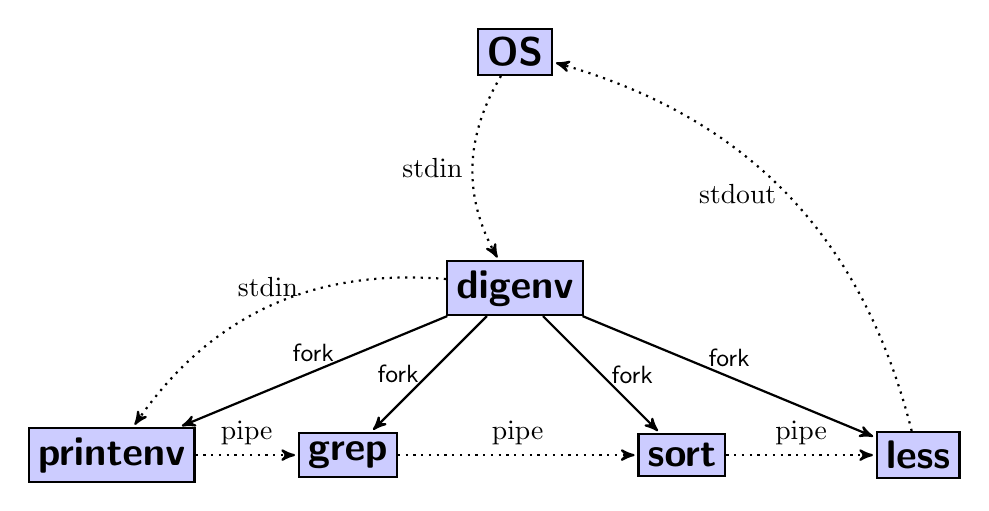
\begin{tikzpicture}[->,>=stealth',shorten >=1pt,auto,node distance=3cm,
  thick,main node/.style={rectangle,fill=blue!20,draw,font=\sffamily\Large\bfseries}]

  \node[main node] (5) {OS};
  \node[main node] (0) [below of=5] {digenv};
  \node[main node] (2) [below left of=0] {grep};
  \node[main node] (3) [below right of=0] {sort};
  \node[main node] (1) [left of=2] {printenv};
  \node[main node] (4) [right of=3] {less};

  \path[dotted]
    (5) edge [bend right] node [left] {stdin} (0)
    (0) edge [bend right] node [above] {stdin} (1)
    (1) edge node [above] {pipe} (2)
    (2) edge node [above] {pipe} (3)
    (3) edge node [above] {pipe} (4)
    (4) edge [bend right] node [left] {stdout} (5);

  \path[every node/.style={font=\sffamily\small}]
    (0) edge node [above] {fork} (1)
        edge node [left] {fork} (2)
        edge node [right] {fork} (3)
        edge node [above] {fork} (4);
    
\end{tikzpicture}

\subsection{Testkörning}

\begin{lstlisting}
$ digenv.exe HOME

> HOME=/home/calle_000
> HOMEDRIVE=C:
> HOMEPATH=\\Users\\calle\_000

$ digenv.exe COM

> COMMONPROGRAMFILES=C:\Program Files\Common Files
> COMPUTERNAME=ZETATWO
> COMSPEC=C:\WINDOWS\system32\cmd.exe
> PATHEXT=.COM;.EXE;.BAT;.CMD;.VBS;.VBE;.JS;.JSE;.WSF;.WSH;.MSC
> VS110COMNTOOLS=C:\Program Files (x86)\Microsoft Visual Studio 11.0\Common7\Tools\
> VS120COMNTOOLS=C:\Program Files (x86)\Microsoft Visual Studio 12.0\Common7\Tools\
\end{lstlisting}


\clearpage
\section{Källkod}
Källkoden går att läsa nedan. Den går också att ladda ner från Github\footnote{\url{https://github.com/ZetaTwo/dd2200-laborationer/blob/master/labb1/src/digenv.c}} och kompileras med "gcc -Wall digenv.c"
\lstinputlisting[style=cstyle]{../src/digenv.c}
\clearpage

\section{Arbetsgång och Utvärdering}

Labben och rapporten har tillsammans tagit ca. 8 timmar. Materialet som fanns att tillgå var rätt bra. Däremot känns det som att det finns ett stort överlapp mellan innehållet i de olika labb-PM och det allmänna labb-PM:et. Jag har blivit mycket bättre införstådd i de systemanrop som används och hur pipes och exec fungerar.

Jag skrev i stora drag fyra versioner av koden innan jag blev nöjd och allt fungerade bra. I den första versionen förstod jag inte att vi skulle använda exec för att utföre respektive delsteg utan började titta på hur man kunde implementera de olika delstegen. Detta övergav jag rätt snabbt då jag insåg att det inte var tanken. Den andra versionen baserades på att varje process forkade en barnprocess i ett led. Alltså att den första processen forkade och körde printenv, den barnprocessen forkade i sin tur och körde grep, etc. Problemet här var då att den första processen inte riktigt kunde veta när den sista processen var klar. Den tredje versionen använde istället en föräldraprocess som forkade flera gånger med hjälp av en rekursiv funktion. När detta fungerade och uppfyllde kraven för labben så snyggade jag till den och skrev den fjärde och sista versionen som baserades på en loop istället för rekursion. Jag skrev mer eller mindre om tail-rekursionen som en loop.

Jag skulle säga att materialet är bra men överlappet gör att man ibland tappar fokus när man läser "det där har jag redan läst" så att man riskerar att missa saker. Det skulle kanske vara bra att flytta ut mer material till ett kompendium om systemanrop, etc. som är ett förkunskapskrav för både labb 1 och 2.

Gällande såvrighet så är jag rätt bekant med C (egentligen C++) så den biten var inte så farlig men vissa systemanrop och att strukturera det bra var lite småklurigt ändå. Kortfattat:

\begin{itemize}
\item Labb-PM: 3
\item Svårighetsgrad: 3
\item Lärorikhet: 4
\end{itemize}


\end{document}